%%% Template originaly created by Karol Kozioł (mail@karol-koziol.net) and modified for ShareLaTeX use

\documentclass[a4paper,11pt]{article}

\usepackage[T1]{fontenc}
\usepackage[utf8]{inputenc}
\usepackage{graphicx}
\usepackage{xcolor}

\renewcommand\familydefault{\sfdefault}
\usepackage{tgheros}
\usepackage[defaultmono]{droidmono}

\usepackage{placeins}
\usepackage{amsmath,amssymb,amsthm,textcomp}
\usepackage{enumerate}
\usepackage{multicol}
\usepackage{tikz}

\usepackage{geometry}
\geometry{left=25mm,right=25mm,%
bindingoffset=0mm, top=20mm,bottom=20mm}


\linespread{1.3}

\newcommand{\linia}{\rule{\linewidth}{0.5pt}}

% custom theorems if needed
\newtheoremstyle{mytheor}
    {1ex}{1ex}{\normalfont}{0pt}{\scshape}{.}{1ex}
    {{\thmname{#1 }}{\thmnumber{#2}}{\thmnote{ (#3)}}}

\theoremstyle{mytheor}
\newtheorem{defi}{Definition}

% my own titles
\makeatletter
\renewcommand{\maketitle}{
\begin{center}
\vspace{2ex}
{\huge \textsc{\@title}}
\vspace{1ex}
\\
\linia\\
\@author \hfill
\vspace{4ex}
\end{center}
}
\makeatother
%%%

% custom footers and headers
\usepackage{fancyhdr}

\pagestyle{fancy}
\lhead{}
\chead{}
\rhead{}
\lfoot{Statistical Modeling}
\cfoot{}
\rfoot{Page \thepage}
\renewcommand{\headrulewidth}{0pt}
\renewcommand{\footrulewidth}{0pt}
%

% code listing settings
\usepackage{listings}
\lstset{
    language=Python,
    basicstyle=\ttfamily\small,
    aboveskip={1.0\baselineskip},
    belowskip={1.0\baselineskip},
    columns=fixed,
    extendedchars=true,
    breaklines=true,
    tabsize=4,
    prebreak=\raisebox{0ex}[0ex][0ex]{\ensuremath{\hookleftarrow}},
    frame=lines,
    showtabs=false,
    showspaces=false,
    showstringspaces=false,
    keywordstyle=\color[rgb]{0.627,0.126,0.941},
    commentstyle=\color[rgb]{0.133,0.545,0.133},
    stringstyle=\color[rgb]{01,0,0},
    numbers=left,
    numberstyle=\small,
    stepnumber=1,
    numbersep=10pt,
    captionpos=t,
    escapeinside={\%*}{*)}
}

%%%----------%%%----------%%%----------%%%----------%%%

\begin{document}

\title{\textbf{{BRAIN SCIENCE STUDY}}}


\author{Nirupam Bidikar-1878058 | Akshit Tandon-1792038 | Rahul Raj Mogili-1900425}


\maketitle

\section*{Construction of Author Networks}

We aim to visualise author networks for USA, Europe, and Australasia. In these networks, each node is a scholar and edges connecting scholars represent joint publications. The purpose of creating these networks is to compute pagerank which is a fundamental factor in evaluating an author's work in research. Below we show our approach and methodology with explanation of the code.

\section*{The Approach}

%%%%%%%%% description %%%%%%%%%%
% ------------ USA NET START ------------ %
For this part of the project, we import dplyr, plyr and data.table libraries. Initially, let's load the brain author csv file and factor it according to the \texttt{scopus\_id}. We conduct the factorization for \texttt{scopus\_id} in brainAuthor and \texttt{scopus\_id}, \texttt{co\_author\_scopus\_id} in brainPubAuthor data frames. Later, we load the CIP\_category csv file given. \newline

\begin{lstlisting}
library(dplyr)
library(plyr)
library(data.table)

brainAuthor <- read.csv("brain_author.csv")
brainAuthor$scopus_id <- as.factor(brainAuthor$scopus_id)
brainPubAuthors <- read.csv("brain_publication_authors.csv")
brainPubAuthors$scopus_id <- as.factor(brainPubAuthors$scopus_id)
brainPubAuthors$co_author_scopus_id <- as.factor(brainPubAuthors$co_author_scopus_id)
#brainPubDetails <- read.csv("brain_publication_details.csv")
cipCatFile <- read.csv("CIP_category.csv")
colnames(cipCatFile) <- c("cip_title", "cip_category")
\end{lstlisting}

We create a node list by creating an inner join from the brainAuthor and CIP\_category by filtering out the minimum publication year that has to be greater than 1960 and number of publications to be greater than 10, as considering less than 10 would make the author look like a PhD student.\newline

\begin{lstlisting}
nodeListInit <- distinct(inner_join(brainAuthor,cipCatFile,by="cip_title")) %>% filter(min_pub_year > 1960) %>% filter(num_publications > 10) %>% select(scopus_id,region,min_pub_year,cip_category,total_deflated_dollar_2010)
\end{lstlisting}

We initiate with the USA node. We filter out the region to be "US/Canada". Since gephi requires an argument of source in the input, we use the 'rn' from the csv file and rename it to 'Source'. \newline

\begin{lstlisting}
#USA NETWORK
usaNode <- unique(nodeListInit %>% filter(region == "US/Canada")) 
setDT(usaNode,keep.rownames = TRUE)[]
names(usaNode)[names(usaNode) == 'rn'] <- 'Source'
write.csv(usaNode,"usanodelist2.csv",row.names = FALSE)
\end{lstlisting}

To create an edge list 'edgeListInit', we apply an inner join for the usaNode and brainPubAuthor. Now, we select the important columns scopus\_id, region, co\_author\_scopus\_id and Source and filter out any redundancies present in the edge list. We now rename the scopus\_id in the usaNode to co\_author\_scopus\_id for using that in the inner join of the usaNode and edgeListInit. To differentiate the two columns 'Source' we use 'Source.x' for 'Target' and 'Source.y' for 'Source'. We now plug these two inputs to gephi and get a visualisation of usaNode with edges. We write the 'Source' and 'Target' columns in a csv format with page ranks. In gephi, we make use of the Giant Component filter which returns the single most highly connected component in the network which is what shown in the figures for all regions as the original network generated is too complex.

\begin{lstlisting}
edgeListInit <- inner_join(usaNode,brainPubAuthors,by="scopus_id") %>% filter(co_author_scopus_id %in% usaNode$scopus_id) %>% filter(scopus_id %in% usaNode$scopus_id) %>% filter(scopus_id != co_author_scopus_id)
edgeListInit <- edgeListInit %>% select(scopus_id,region,co_author_scopus_id,Source)
edgeListInit <- unique(edgeListInit)

names(usaNode)[names(usaNode) == 'scopus_id'] <- 'co_author_scopus_id'
edgeListInit <- inner_join(usaNode,edgeListInit,by="co_author_scopus_id")

names(edgeListInit)[names(edgeListInit) == 'Source.y'] <- 'Target'
names(edgeListInit)[names(edgeListInit) == 'Source.x'] <- 'Source'

usaEdgeList <- edgeListInit  %>% select(Source,Target)
write.csv(usaEdgeList,"usaedgelist2.csv",row.names = FALSE)
\end{lstlisting}

\begin{figure}[ht]
    \centering
    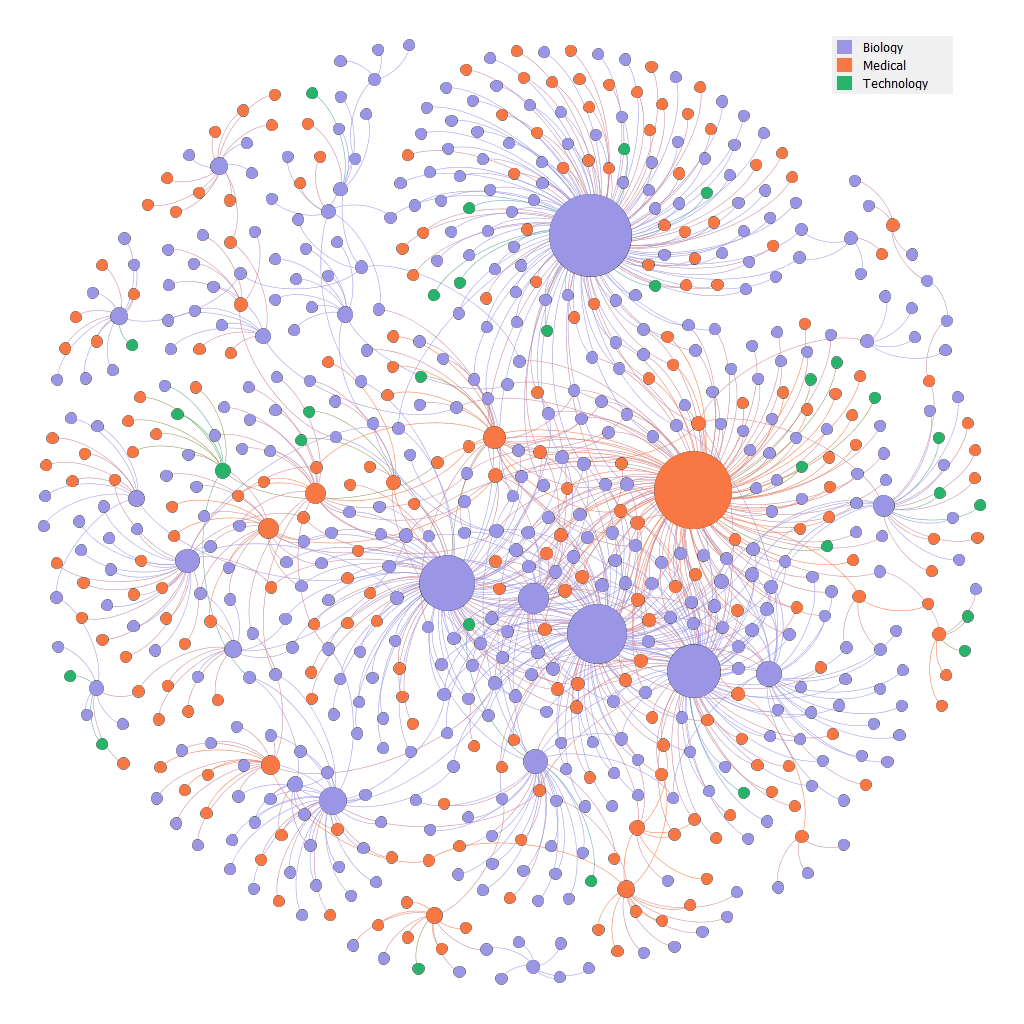
\includegraphics[width=15cm]{usanet_legend2.png}
    \caption{USA Network}
    \label{fig:USA Network}
\end{figure}

With respect to the fig \ref{fig:USA Network}, we can observe two authors with highest number of co authors each from Biology and Medical. Apart from that, Biology has more than half number of nodes followed by Medical and the least being Technology.  \newline

% ------------ USA NET END ------------ %
% ------------ EUROPE NET START ------------ %


We do similar implementations for Europe by replacing the region filter to 'Europe'.   

\begin{lstlisting}
#EUROPE NETWORK
europeNode <- nodeListInit %>% filter(region == "Europe") 
setDT(europeNode,keep.rownames = TRUE)[]
names(europeNode)[names(europeNode) == 'rn'] <- 'Source'
write.csv(europeNode,"europeNodelist.csv",row.names = FALSE)

europeEdgeList <- inner_join(europeNode,brainPubAuthors,by="scopus_id") %>% filter(co_author_scopus_id %in% europeNode$scopus_id) %>% filter(scopus_id %in% europeNode$scopus_id) %>% filter(scopus_id != co_author_scopus_id)
europeEdgeList <- europeEdgeList %>% select(scopus_id,region,co_author_scopus_id,Source)
europeEdgeList <- unique(europeEdgeList)

names(europeNode)[names(europeNode) == 'scopus_id'] <- 'co_author_scopus_id'
europeEdgeList <- inner_join(europeNode,europeEdgeList,by="co_author_scopus_id")

names(europeEdgeList)[names(europeEdgeList) == 'Source.y'] <- 'Target'
names(europeEdgeList)[names(europeEdgeList) == 'Source.x'] <- 'Source'
europeEdgeList <- europeEdgeList %>% select(Source,Target)
write.csv(europeEdgeList,"europeEdgeList.csv",row.names = F)
\end{lstlisting}

\begin{figure}[ht]
    \centering
    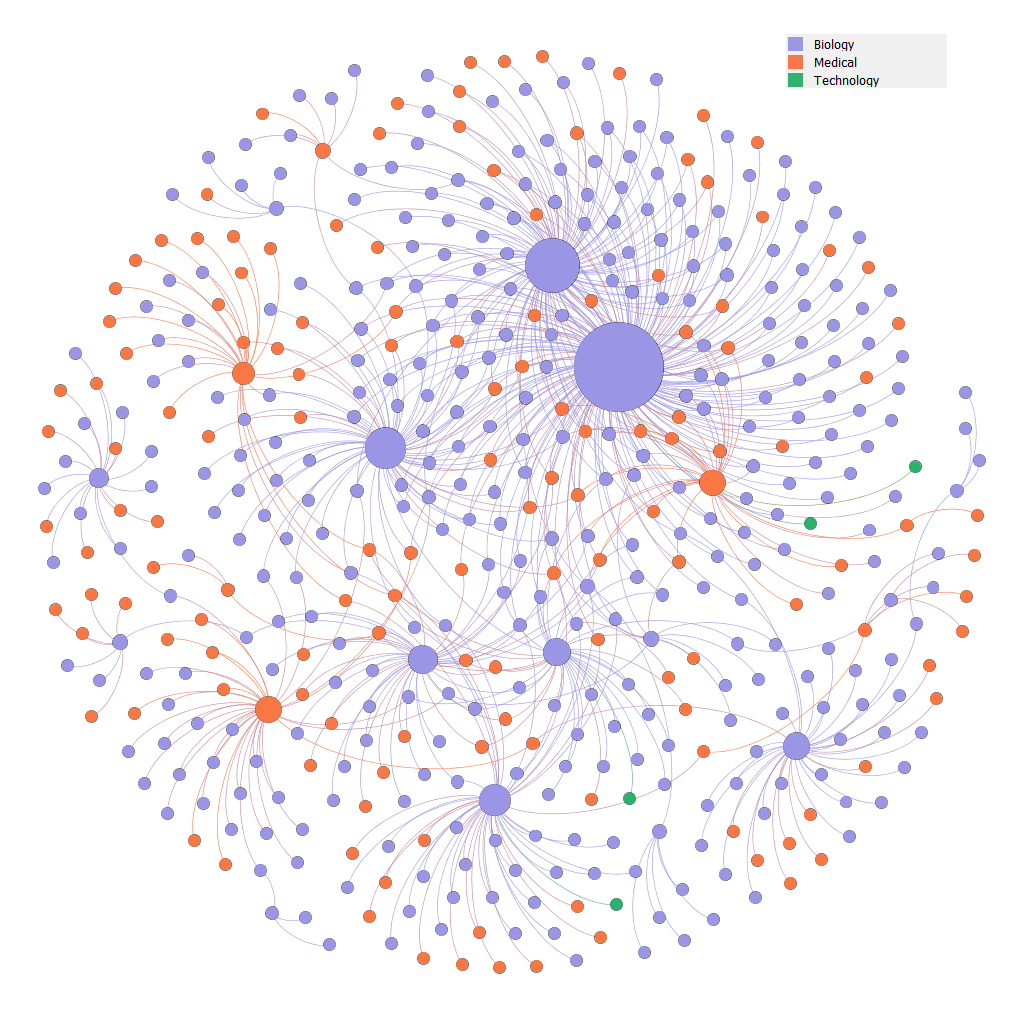
\includegraphics[width=15cm]{europenet_legend2.png}
    \caption{EUROPE Network}
    \label{fig:EUROPE Network}
\end{figure} \newpage

From fig \ref{fig:EUROPE Network}, we can observe that, Biology unanimously outnumbered Medical and Technology in terms of networking. Technology department has very few edges. \newline

% ------------ EUROPE NET END ------------ %
% ------------ AUSTRALASIA NET START ------------ %
We do similar implementations for Australasia by replacing the region filter to 'Australasia'.

\begin{lstlisting}
#AUSTRALASIA NETWORK
australasiaNodeList <- nodeListInit %>% filter(region == "Australasia")
setDT(australasiaNodeList,keep.rownames = TRUE)[]
names(australasiaNodeList)[names(australasiaNodeList) == 'rn'] <- 'Source'
write.csv(australasiaNodeList,"australasiaNodelist.csv",row.names = FALSE)

australasiaEdgeList <- inner_join(australasiaNodeList,brainPubAuthors,by="scopus_id") %>% filter(co_author_scopus_id %in% australasiaNodeList$scopus_id) %>% filter(scopus_id %in% australasiaNodeList$scopus_id) %>% filter(scopus_id != co_author_scopus_id)
australasiaEdgeList <- australasiaEdgeList %>% select(scopus_id,region,co_author_scopus_id,Source)
australasiaEdgeList <- unique(australasiaEdgeList)

names(australasiaNodeList)[names(australasiaNodeList) == 'scopus_id'] <- 'co_author_scopus_id'
australasiaEdgeList <- inner_join(australasiaNodeList,australasiaEdgeList,by="co_author_scopus_id")

names(australasiaEdgeList)[names(australasiaEdgeList) == 'Source.y'] <- 'Target'
names(australasiaEdgeList)[names(australasiaEdgeList) == 'Source.x'] <- 'Source'
australasiaEdgeList <- australasiaEdgeList %>% select(Source,Target)
write.csv(australasiaEdgeList,"australasiaEdgeList.csv",row.names = F)
\end{lstlisting} \newpage

\begin{figure}[ht]
    \centering
    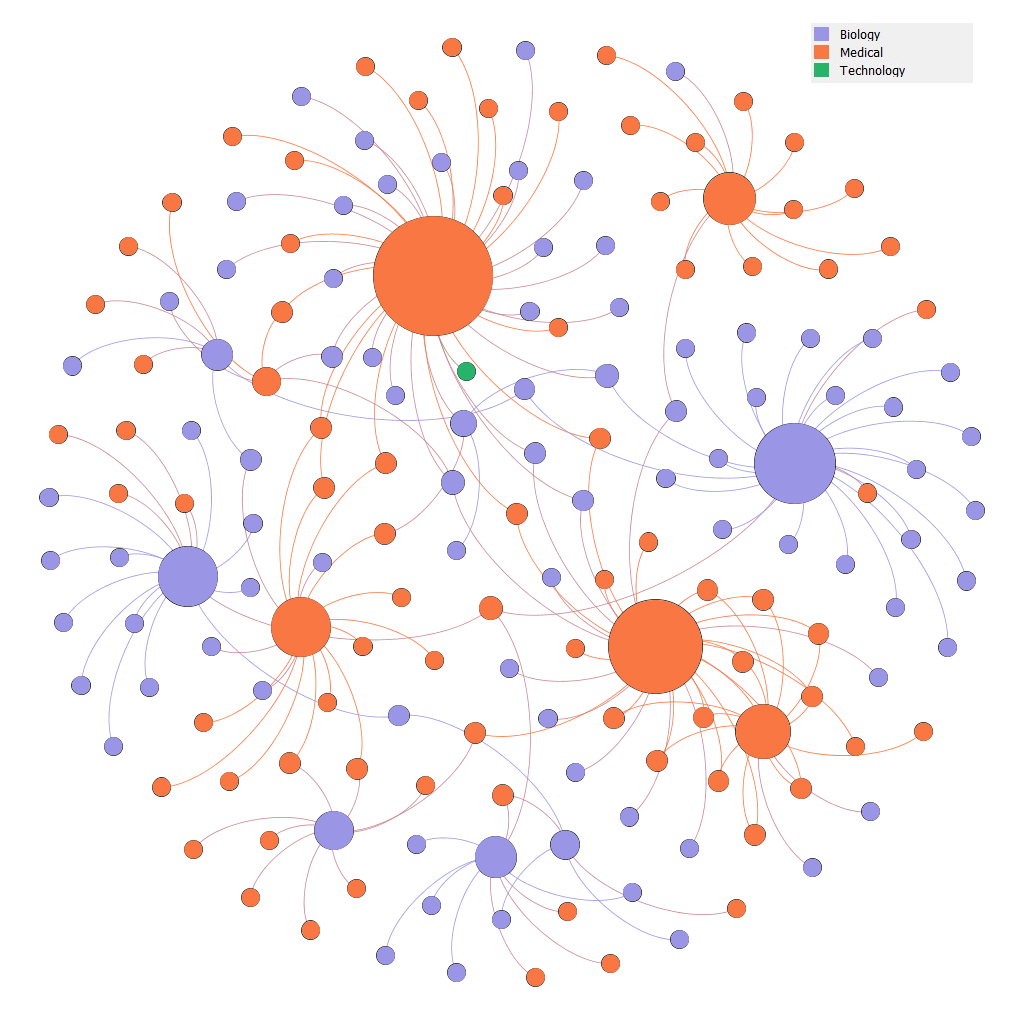
\includegraphics[width=15cm]{australianet_legend2.png}
    \caption{AUSTRALASIA Network}
    \label{fig:AUSTRALASIA Network}
\end{figure}

From fig \ref{fig:AUSTRALASIA Network}, we can observe that Biology and Medical have almost same number of edges. Medical has bigger nodes compared to Biology. Even in this region, Technology has least number of edges. \newline

% ------------ AUSTRALASIA NET END ------------ %

With the observations from \ref{fig:USA Network}, \ref{fig:EUROPE Network} and \ref{fig:EUROPE Network}, we can say that USA has the most number of authors followed by Europe and Australasia region being the least. We can also see from the networks that researchers mostly collaborate with other researches from the same field.
\section*{Fitting Linear Models}

Here, we aim to develop 3 multiple regressions models, one for each geographic area - USA, Europe, and Australasia which help us predict the success of a researcher based on several attributes. The key predictor variable is cross-disciplinarity and the response variable being total citations. Our primary idea is to find the relationship between cross disciplinarity and success. We also investigate if cross disciplinary research translates to greater success. We use the following base equation to construct the models and choose varying attributes for different regions due to unavailability of data.

\begin{multline*}
    log(citations) = log(1+deptRank) + log(1+funding) + log(1+pagerank) +\\
    cipCategory + AgeVariation
\end{multline*}
  
We also use a stricter model with an author being considered if he has 4 or more links with authors from different fields. The construction and subsequent analysis is elaborated below.
\section*{Developing Linear Models}

% ------------ USA MODEL START ------------ %
For this part of analysis, we import dplyr, plyr, data.table and GGally libraries. Initially let's start with the USA model. We generate the page rank file from gephi and load it along with the USA node csv file and do an inner\_join between the page rank and the node file with respect to scopus\_id. 

\begin{lstlisting}
library(dplyr)
library(plyr)
library(data.table)
library("GGally")

#USA MODEL
pagerank <- read.csv("usapagerank2.csv")
cdfile <- read.csv("usa-nodes.csv")
pagerankwithcd <- inner_join(pagerank,cdfile,by="scopus_id")
\end{lstlisting}

Now, within the data frame, let us remove additional columns like Label, timeset, cip\_category.x, minimum publication year and the number of funds.  Factor the cip\_category and y\_05 columns and mutate them.

\begin{lstlisting}
new <- within(pagerankwithcd, rm(Label,timeset,cip_category.x,min_pub_year,X,num_of_fund))
new$cip_category <- as.factor(new$cip_category.y)
new$y_05 <- as.factor(new$y_05)
new <- new %>% mutate(y_05 = relevel(y_05, ref = "1960"))
\end{lstlisting}

We set 'NA' values in the data frame to 0 for funding and ignore the rows if their department rank is null. Now, let us run a linear model on the citations, cross disciplinarity, dept\_rank, total\_deflated\_dollar\_2010, pageranks, cip\_category, y\_05 corresponding with the 'new' data frame. Summarize the results. Finally, set up a matrix of plots using 'ggpairs'.

From fig \ref{fig:USA CORRELATION}, we can infer the following interpretations. We observe the total\_deflated\_dollar\_2010, citations and pageranks to be exponential. We also see that Biology has most number of publications followed by Medical and Technology. In spite of Medical having less number of publications compared to Biology, it's dept\_rank is more significant compared to the other two departments. 

\begin{lstlisting}
#usa model
new$y_05 <- as.factor(new$y_05)
new <- new %>% mutate(y_05 = relevel(y_05, ref = "2015"))
new <- new %>% filter(!is.na(dept_rank))
new$total_deflated_dollar_2010[is.na(new$total_deflated_dollar_2010)] = 0
usamodel <- lm(log(1 +citations) ~  factor(CD) + log(1+dept_rank) +log(1+total_deflated_dollar_2010) + log(1+pageranks)+  cip_category + y_05 ,data=new)
summary(usamodel)

graphframe <- new %>% select (total_deflated_dollar_2010, pageranks, citations, cip_category, dept_rank) %>% filter(!is.na(dept_rank))
ggpairs(graphframe,aes(col = cip_category, alpha=0.4))

#usa  strict model 

new$cip_category <- as.factor(new$cip_category.y)
new <- new %>% mutate(cip_category = relevel(cip_category, ref = "Technology"))
new$y_05 <- as.factor(new$y_05)
new <- new %>% mutate(y_05 = relevel(y_05, ref = "2015"))
new <- new %>% filter(!is.na(dept_rank))
new$total_deflated_dollar_2010[is.na(new$total_deflated_dollar_2010)] = 0
usamodel <- lm(log(1 +citations) ~  factor(Stricter_CD) + log(1+dept_rank) +log(1+total_deflated_dollar_2010) + log(1+pageranks)+  cip_category + y_05 ,data=new)
summary(usamodel)
graphframe <- new %>% select (total_deflated_dollar_2010, pageranks, citations, cip_category, dept_rank) %>% filter(!is.na(dept_rank))
ggpairs(graphframe,aes(col = cip_category, alpha=0.4))

\end{lstlisting} 

\newpage

\begin{figure}[h]
    \centering
    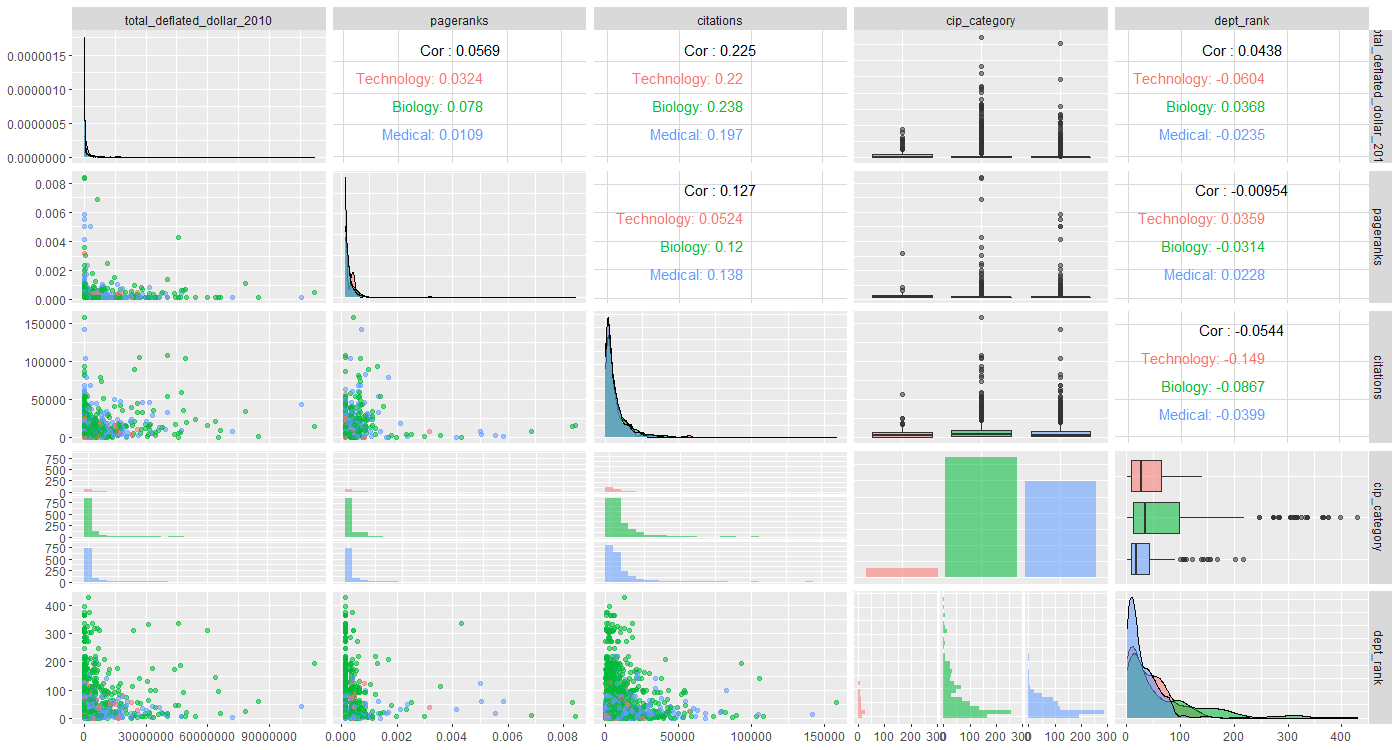
\includegraphics[width=16cm, height=16cm]{usa_nonstrict_cor.png}
    \caption{USA CORRELATION}
    \label{fig:USA CORRELATION}
\end{figure} 

We also implemented a stricter cross disciplinary model for the USA region, as shown in fig \ref{fig:USA BASE MODEL}. We observe that there are minute changes in the coefficients with the estimates increasing in the stricter cross disciplinary model. \newpage 

\begin{figure}[h]
    \centering
    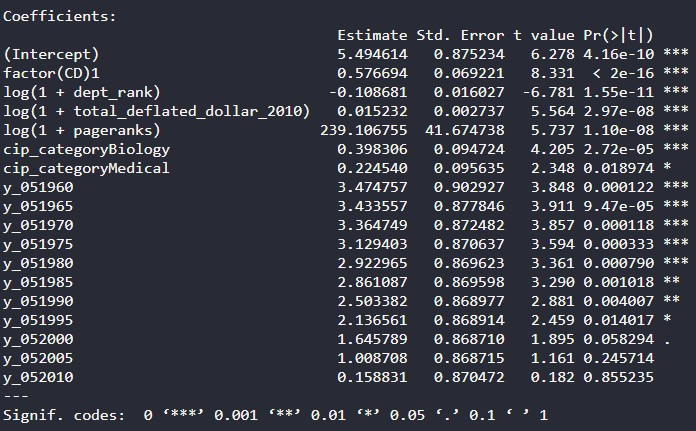
\includegraphics[width=16cm, height=10cm]{usa_coeff_non.jpg}
    \caption{USA BASE MODEL}
    \label{fig:USA BASE MODEL}
\end{figure}
\FloatBarrier

In both base model  (fig \ref{fig:USA BASE MODEL}) and the stricter model (fig \ref{fig:USA STRICT CORRELATION}), we see pagerank being extremely significant. We can also observe a decreasing trend in the coefficient values of the age factor which translates to the fact that authors who have recently started publishing research are less likely to be more successful. Department rank has a negative coefficient showing greater the rank lesser the significance. Biology and Medical fields show significance which indicates that an author belonging to these fields is more likely to be successful. Cross disciplinarity is another significant factor but has a lesser value than pagerank and age factor. Funding turns out to be a significant attribute but the coefficient suggests it's not a big influence on the response variable. \\

\begin{figure}[h]
    \centering
    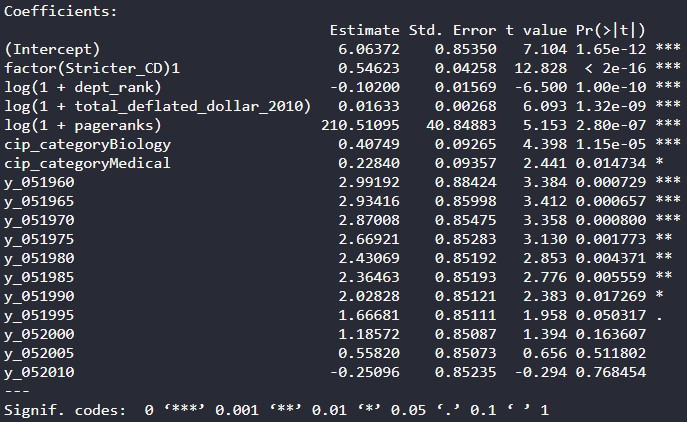
\includegraphics[width=16cm, height=10cm]{usa_coeff_str.jpg}
    \caption{USA MODEL WITH STRICT CD}
    \label{fig:USA STRICT CORRELATION}
\end{figure} 
\FloatBarrier



% ------------ USA MODEL END ------------ %
% ------------ EUROPE MODEL START ------------ %

We do similar implementations for Europe with Page rank csv file of Europe. Here we drop the department rank attribute due to unavailability of data.

\begin{lstlisting}
#europe model

eucomb$cip_category.y <- as.factor(eucomb$cip_category.y)
eucomb$y_05 <- as.factor(eucomb$y_05)
eucomb <- eucomb %>% mutate(cip_category.y = relevel(cip_category.y, ref = "Technology"))
eucomb <- eucomb %>% mutate(y_05 = relevel(y_05, ref = "2015"))
europemodel <-  lm(log(1 +citations) ~  factor(CD) +log(1+total_deflated_dollar_2010) + log(1+pageranks)+  cip_category.y + y_05 ,data=eucomb)
summary(europemodel)

graphframe <- eucomb %>% select (total_deflated_dollar_2010, pageranks, citations, cip_category.y) 
ggpairs(graphframe,aes(col = cip_category.y, alpha=0.4))
#europe stricter model

eucomb$cip_category.y <- as.factor(eucomb$cip_category.y)
eucomb$y_05 <- as.factor(eucomb$y_05)
eucomb <- eucomb %>% mutate(cip_category.y = relevel(cip_category.y, ref = "Technology"))
eucomb <- eucomb %>% mutate(y_05 = relevel(y_05, ref = "2015"))
eucomb$total_deflated_dollar_2010[is.na(eucomb$total_deflated_dollar_2010)] = 0
europemodel <-  lm(log(1 +citations) ~  factor(Stricter_CD) +log(1+total_deflated_dollar_2010) + log(1+pageranks)+  factor(cip_category.y) + factor(y_05) ,data=eucomb)
summary(europemodel)
graphframe <- eucomb %>% select (total_deflated_dollar_2010, pageranks, citations, cip_category.y) 
ggpairs(graphframe,aes(col = cip_category.y, alpha=0.4))
\end{lstlisting}

\begin{figure}[h]
    \centering
    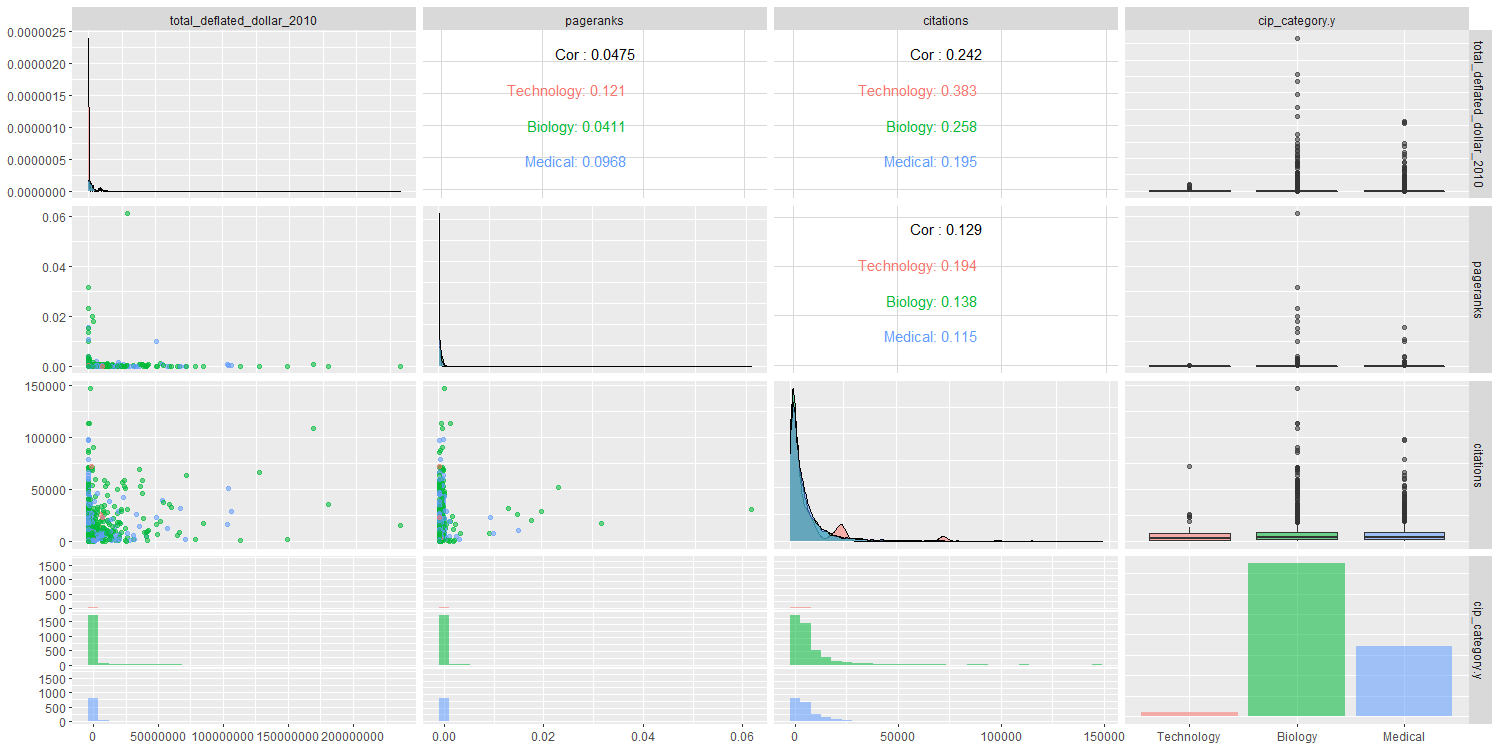
\includegraphics[width=16cm, height=14cm]{eur_nonstrict_cor.png}
    \caption{EUROPE CORRELATION}
    \label{fig:EUROPE CORRELATION}
\end{figure} 

\begin{figure}[h]
    \centering
    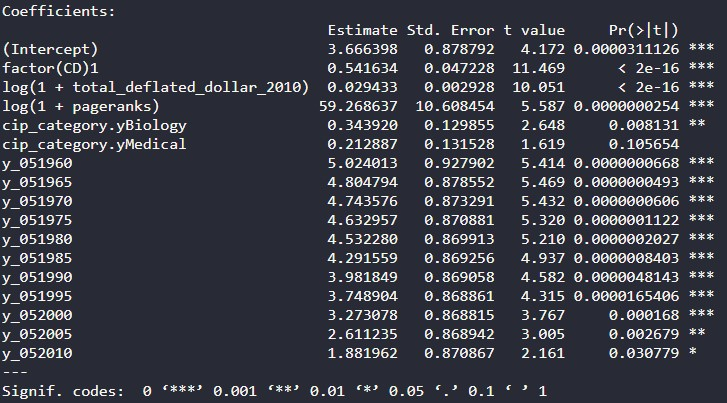
\includegraphics[width=16cm, height=10cm]{europe_coeff_non.jpg}
    \caption{EUROPE BASE MODEL}
    \label{fig:EUROPE BASE CORRELATION}
\end{figure} 

\begin{figure}[h]
    \centering
    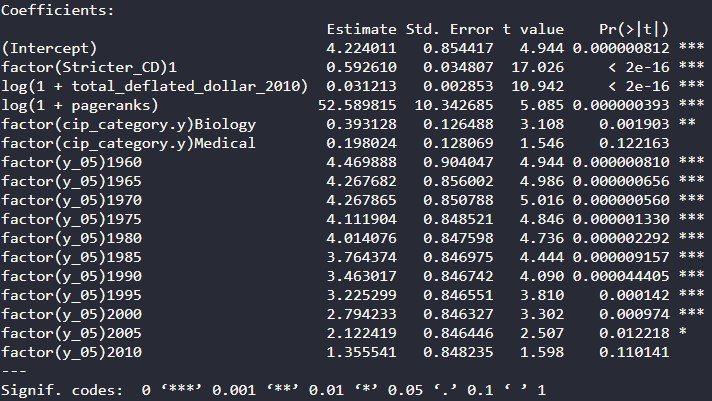
\includegraphics[width=16cm, height=10cm]{europe_coeff_str.jpg}
    \caption{EUROPE MODEL WITH STRICT CD}
    \label{fig:EUROPE STRICT CORRELATION}
\end{figure} 
\FloatBarrier
\newpage
Similar to USA, we can see a decreasing trend in the coefficients as well. The page rank values for both the base model (fig \ref{fig:EUROPE BASE CORRELATION}) and strict CD model (fig \ref{fig:EUROPE STRICT CORRELATION}) are highly significant. We can also observe there are no negative coefficients, like the USA model. Biology and Medical show a good amount of significance stating that authors who worked for these fields are likely to be successful. Additionally, funding has a contributing factor on the significance but has less weight on the response variable. Cross-disciplinarity is on the positive side and we can observe it increases from the base model to stricter model but, like the funding, has no high influence on the model. \\

% ------------ EUROPE MODEL END ------------ %
% ------------ AUSTRALASIA MODEL START ------------ %

We do similar implementation for Australasia with Page rank csv file of Australasia.

\begin{lstlisting}
#australasia model


auscomb$y_05 <- as.factor(auscomb$y_05)
auscomb <- auscomb %>% mutate(cip_category.y = relevel(cip_category.y, ref = "Technology"))
auscomb <- auscomb %>% mutate(y_05 = relevel(y_05, ref = "2015"))
auscomb$total_deflated_dollar_2010[is.na(auscomb$total_deflated_dollar_2010)] = 0
ausmodel <- lm(log(1 +citations) ~  factor(CD)  + log(1+pageranks)+  cip_category.y + y_05 ,data=auscomb)
summary(ausmodel)
graphframe <- auscomb %>% select  (pageranks, citations, cip_category.y) 
ggpairs(graphframe,aes(col = cip_category.y, alpha=0.4))

#australia strict model

auscomb$cip_category.y <- as.factor(auscomb$cip_category.y)
auscomb$y_05 <- as.factor(auscomb$y_05)
auscomb <- auscomb %>% mutate(cip_category.y = relevel(cip_category.y, ref = "Technology"))
auscomb <- auscomb %>% mutate(y_05 = relevel(y_05, ref = "2015"))
auscomb$total_deflated_dollar_2010[is.na(auscomb$total_deflated_dollar_2010)] = 0
ausmodel <- lm(log(1 +citations) ~  factor(Stricter_CD) +log(1+total_deflated_dollar_2010) + log(1+pageranks)+  factor(cip_category.y) + factor(y_05) ,data=auscomb)
summary(ausmodel)
graphframe <- auscomb %>% select  (pageranks, citations, cip_category.y) 
ggpairs(graphframe,aes(col = cip_category.y, alpha=0.4))
\end{lstlisting}

\begin{figure}[ht]
    \centering
    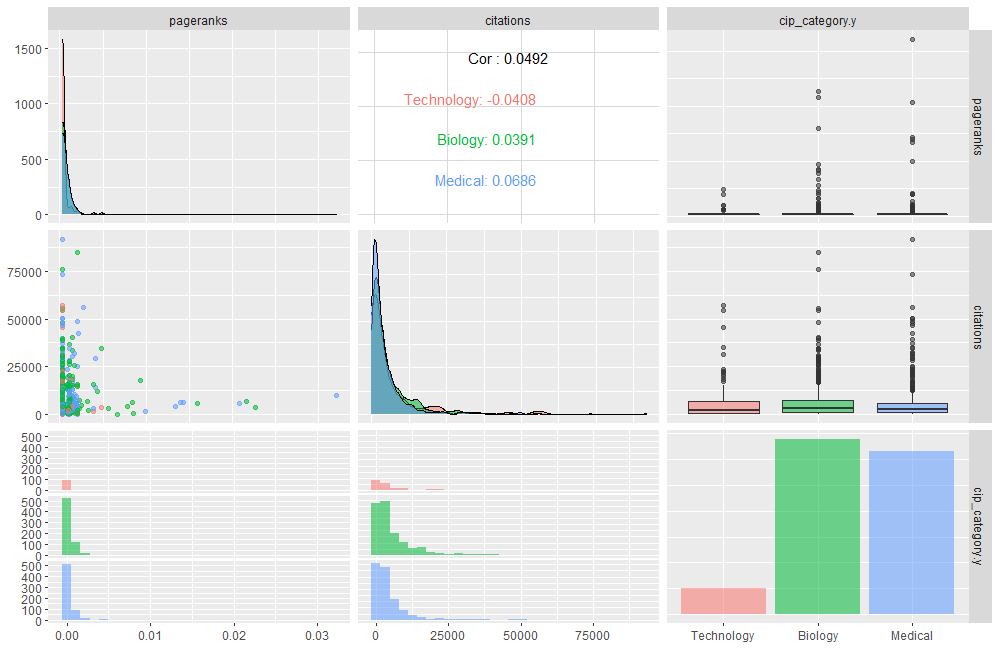
\includegraphics[width=16cm, height=16cm]{aus_nonstrict_cor.png}
    \caption{AUSTRALASIA CORRELATION}
    \label{fig:AUSTRALASIA CORRELATION}
\end{figure}
\newpage
\begin{figure}[ht]
    \centering
    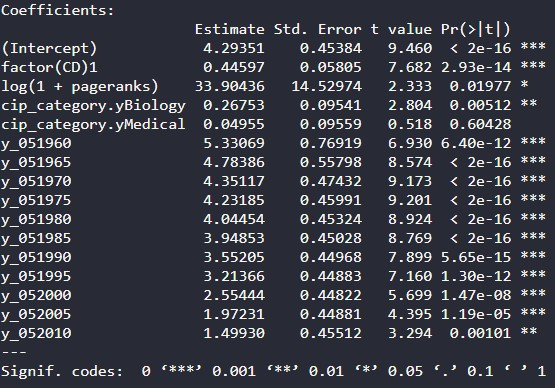
\includegraphics[width=16cm, height=10cm]{aus_coeff_non.jpg}
    \caption{AUSTRALASIA BASE MODEL}
    \label{fig:AUSTRALASIA BASE CORRELATION}
\end{figure} 
\newpage
\begin{figure}[ht]
    \centering
    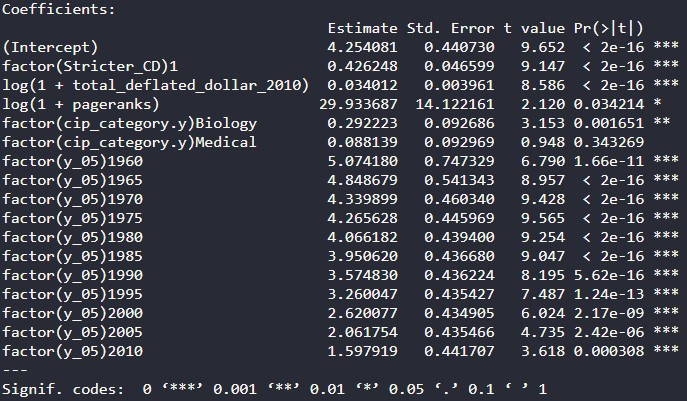
\includegraphics[width=16cm, height=10cm]{aus_coeff_str.jpg}
    \caption{AUSTRALASIA MODEL WITH STRICT CD}
    \label{fig:AUSTRALASIA STRICT CORRELATION}
\end{figure} 
\FloatBarrier

For the Australasia region, we notice that the pagerank is less significant when compared to US, Europe. We again see a decreasing trend in coefficient values as the year values increase which coincides with our findings from the previous models. Medical field turns out to be insignificant in this region and cross disciplinarity continues to have a positive impact. 
% ------------ AUSTRALASIA MODEL END ------------ %

\section*{Conclusion}

After looking through six different models - two for each region, we have seen that pagerank had the most significant impact on the success factor. We have seen commonalities in models with the trends in years, cross disciplinarity and, importance of Biology field. \\
In the stricter model, we observe a slight reduction in the coefficient values for cross discipline with the exception of Europe, but the residual errors value have dropped compared to the base models telling us that the stricter model is a slightly better fit for the data. Cross disciplinary research produces greater technological advancements and accelerates the growth of all the fields involved in the research. This will lead us to believe that it has to be an extremely significant factor in the success of a researcher. From our models we find that it is a significant attribute but is overshadowed by pagerank and the amount of years the author has spent in research. Given this is a multi linear regression model, there is interplay between many factors which may be causing cross disciplinarity to have a lesser significance.
\newline
Secondly, we see a decreasing trend in Age i.e. the estimate value decreases as the year increase starting from 1960 to 2015. Hence, it can be concluded that researchers who have recently started publishing are likely to be less successful than researchers who started back in the 1960's.

\end{document}
